\documentclass{article}
\usepackage[T1]{fontenc} % Enhanced font encoding
\usepackage[utf8]{inputenc} % UTF-8 encoding
\usepackage{amsmath}
\usepackage{graphicx}
\usepackage{hyperref}
\usepackage{listings}
\usepackage{enumitem}
\usepackage{geometry}
\usepackage{float}
\usepackage{booktabs}
\usepackage{subfigure} % Consider replacing with subcaption for modern documents
\usepackage{svg}

% Set page margins
\geometry{
    a4paper,
    top=2.5cm,
    bottom=2.5cm,
    left=2.5cm,
    right=2.5cm
}

% Configure hyperref
\hypersetup{
    colorlinks=true,
    linkcolor=blue,
    filecolor=magenta,
    urlcolor=cyan,
}

% Custom commands
\newcommand{\figref}[1]{Figure~\ref{#1}}
\newcommand{\secref}[1]{Section~\ref{#1}}

\title{\textbf{Conditional Variational Autoencoder (CVAE): \\
Architecture and Implementation Analysis}}
\author{Technical Report}
\date{\today}

\begin{document}

\maketitle

\begin{abstract}
This technical report presents a detailed analysis of the Conditional Variational Autoencoder (CVAE) architecture, focusing on its structural components, operational workflow, and architectural considerations. The CVAE extends traditional VAE capabilities by incorporating conditional information in both encoding and decoding processes, specifically designed for modeling relationships between positions and momenta in high-dimensional spaces. Through comprehensive examination of its components and training results, this report provides insights into the architecture's design choices, implementation features, operational characteristics, and performance metrics.
\end{abstract}

\tableofcontents
\newpage

\section{Introduction}
The Conditional Variational Autoencoder (CVAE) represents an advanced extension of the standard VAE framework, incorporating conditional information to enhance generative capabilities. This implementation specifically targets the modeling of position-momentum relationships, enabling the generation of position data conditioned on specific momentum inputs.

\begin{figure}[H]
    \centering
    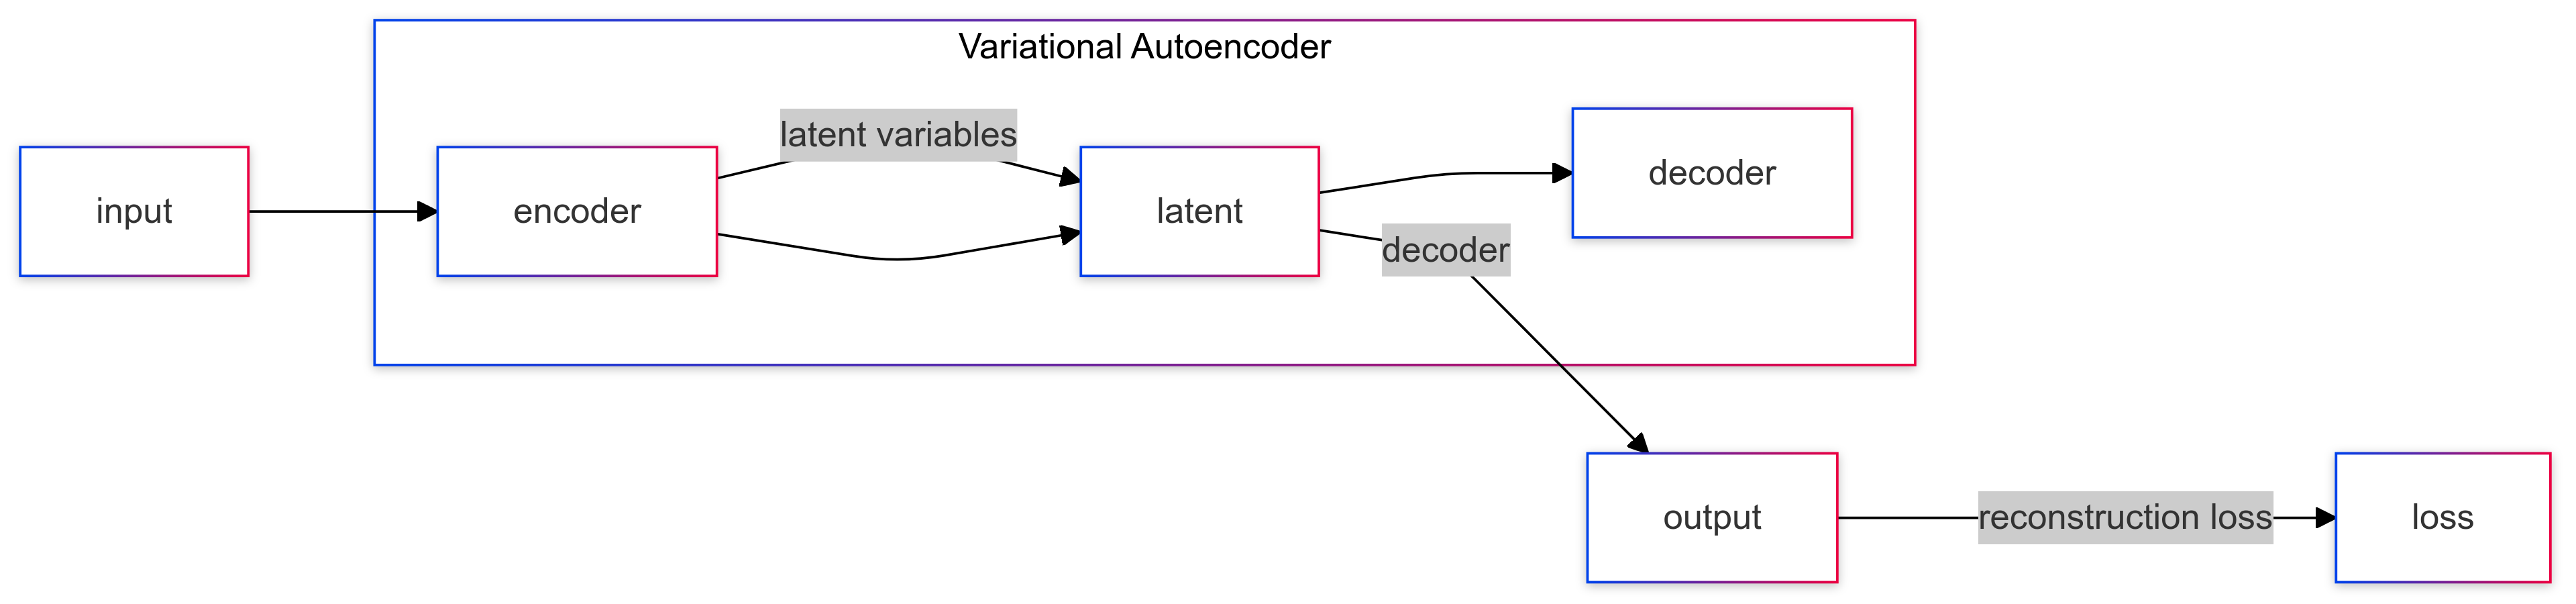
\includegraphics[width=0.8\textwidth]{1.png}
    \caption{Basic Variational Autoencoder Architecture: High-level overview showing the core components including input, encoder, latent space, decoder, output, and loss computation. The diagram highlights the flow of latent variables and the reconstruction loss pathway.}
    \label{fig:architecture}
\end{figure}

\section{Architectural Components}

\subsection{Encoder}
The encoder transforms 9-dimensional input positions into a latent representation with the following specific architecture:
\begin{itemize}
    \item \textbf{Input Layer:} 9-dimensional position vectors
    \item \textbf{Hidden Layer 1:} Linear transformation ($9 \rightarrow 1152$) followed by ReLU activation
    \item \textbf{Hidden Layer 2:} Linear transformation ($1152 \rightarrow 1152$) followed by ReLU activation
    \item \textbf{Output Branches:}
    \begin{itemize}
        \item Mean ($\mu$) computation: Linear layer ($1152 \rightarrow 1920$)
        \item Log variance ($\log\sigma^2$) computation: Linear layer ($1152 \rightarrow 1920$)
    \end{itemize}
\end{itemize}

\begin{figure}[H]
    \centering
    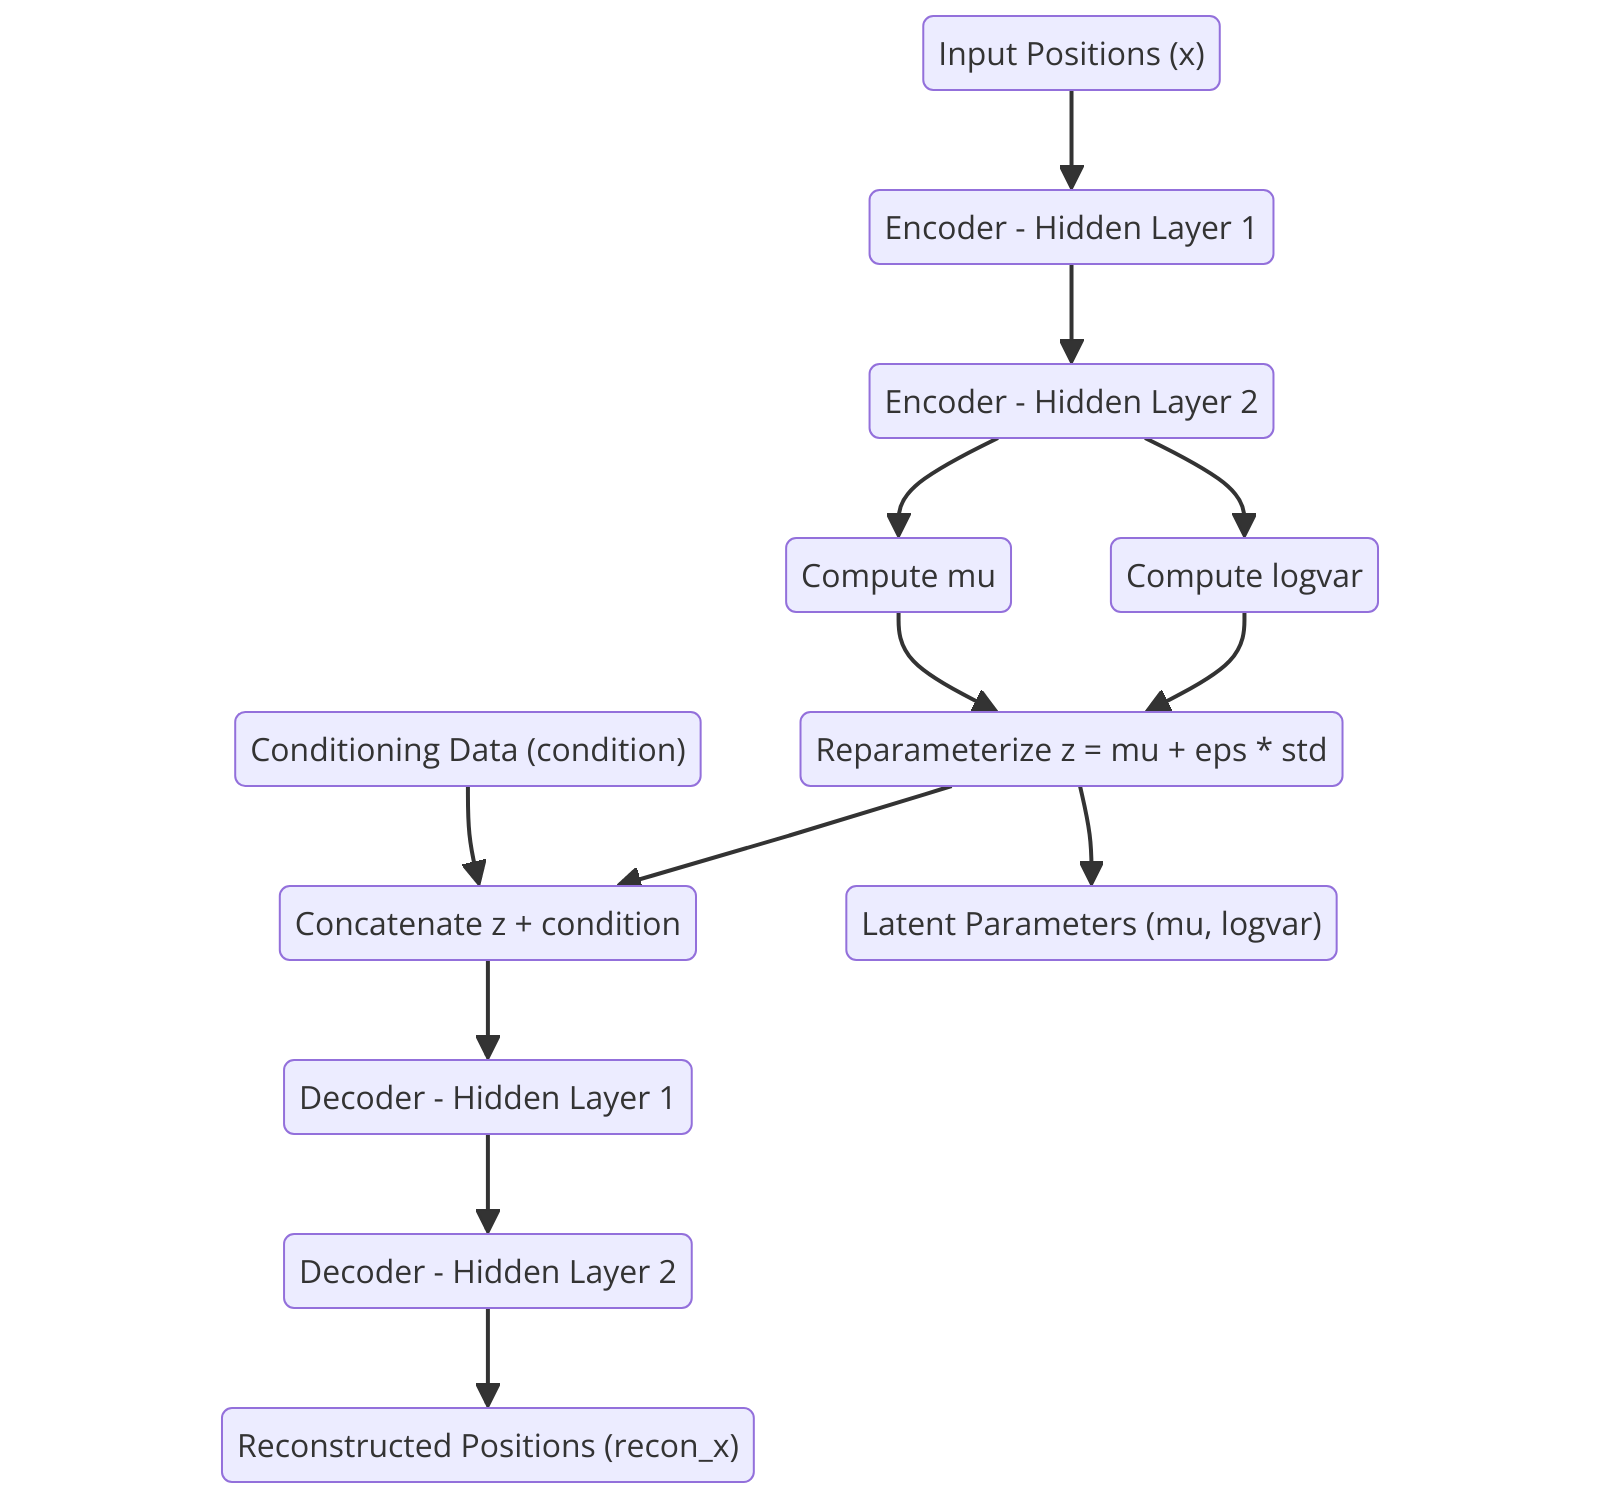
\includegraphics[width=0.7\textwidth]{2.png}
    \caption{Detailed CVAE Flow Diagram: Step-by-step visualization of the complete process, from input positions through encoder layers, computation of latent parameters, reparameterization, conditioning data integration, and decoder reconstruction.}
    \label{fig:flow}
\end{figure}

\subsection{Latent Space and Reparameterization}
The latent space implementation includes:
\begin{itemize}
    \item \textbf{Dimensionality:} 1920-dimensional space
    \item \textbf{Reparameterization:} $z = \mu + \epsilon \cdot \sigma$, where:
    \begin{itemize}
        \item $\epsilon \sim \mathcal{N}(0, I)$
        \item $\sigma = \exp\left(\frac{\log\sigma^2}{2}\right)$
    \end{itemize}
    \item \textbf{Conditioning Integration:} Concatenation of $z$ (1920D) with condition (9D) resulting in a 1929D vector
\end{itemize}

\begin{figure}[H]
    \centering
    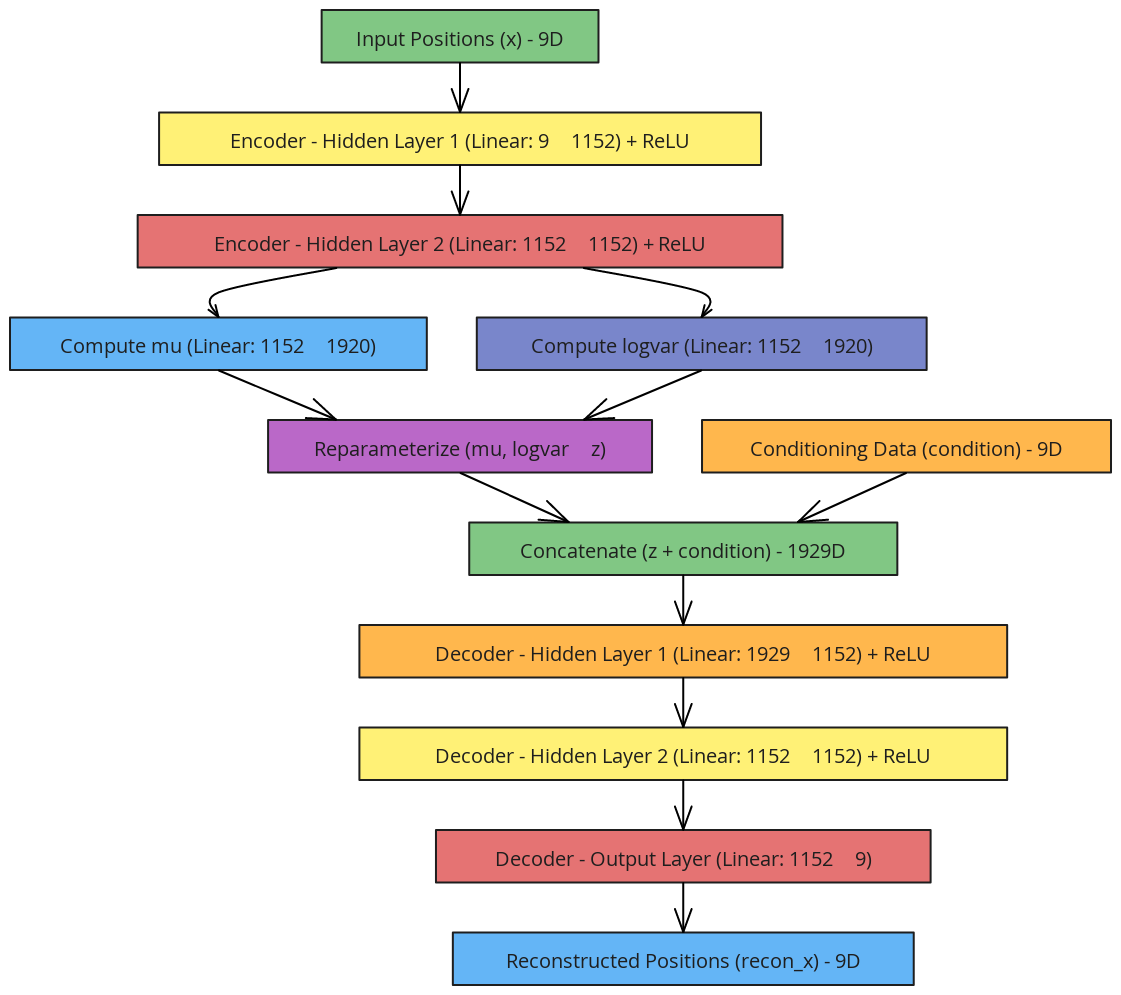
\includegraphics[width=0.7\textwidth]{3.png}
    \caption{Detailed Network Architecture: Complete visualization of the network showing exact layer dimensions and transformations, including the 9D input, 1152-neuron hidden layers, 1920D latent space, and the conditioning mechanism.}
    \label{fig:detailed_architecture}
\end{figure}

\subsection{Decoder}
The decoder architecture precisely mirrors the encoder in reverse, with specific dimensions:
\begin{itemize}
    \item \textbf{Input:} 1929-dimensional concatenated vector (1920D latent + 9D condition)
    \item \textbf{Hidden Layer 1:} Linear transformation ($1929 \rightarrow 1152$) with ReLU
    \item \textbf{Hidden Layer 2:} Linear transformation ($1152 \rightarrow 1152$) with ReLU
    \item \textbf{Output Layer:} Linear transformation ($1152 \rightarrow 9$) for position reconstruction
\end{itemize}

\begin{figure}[H]
    \centering
    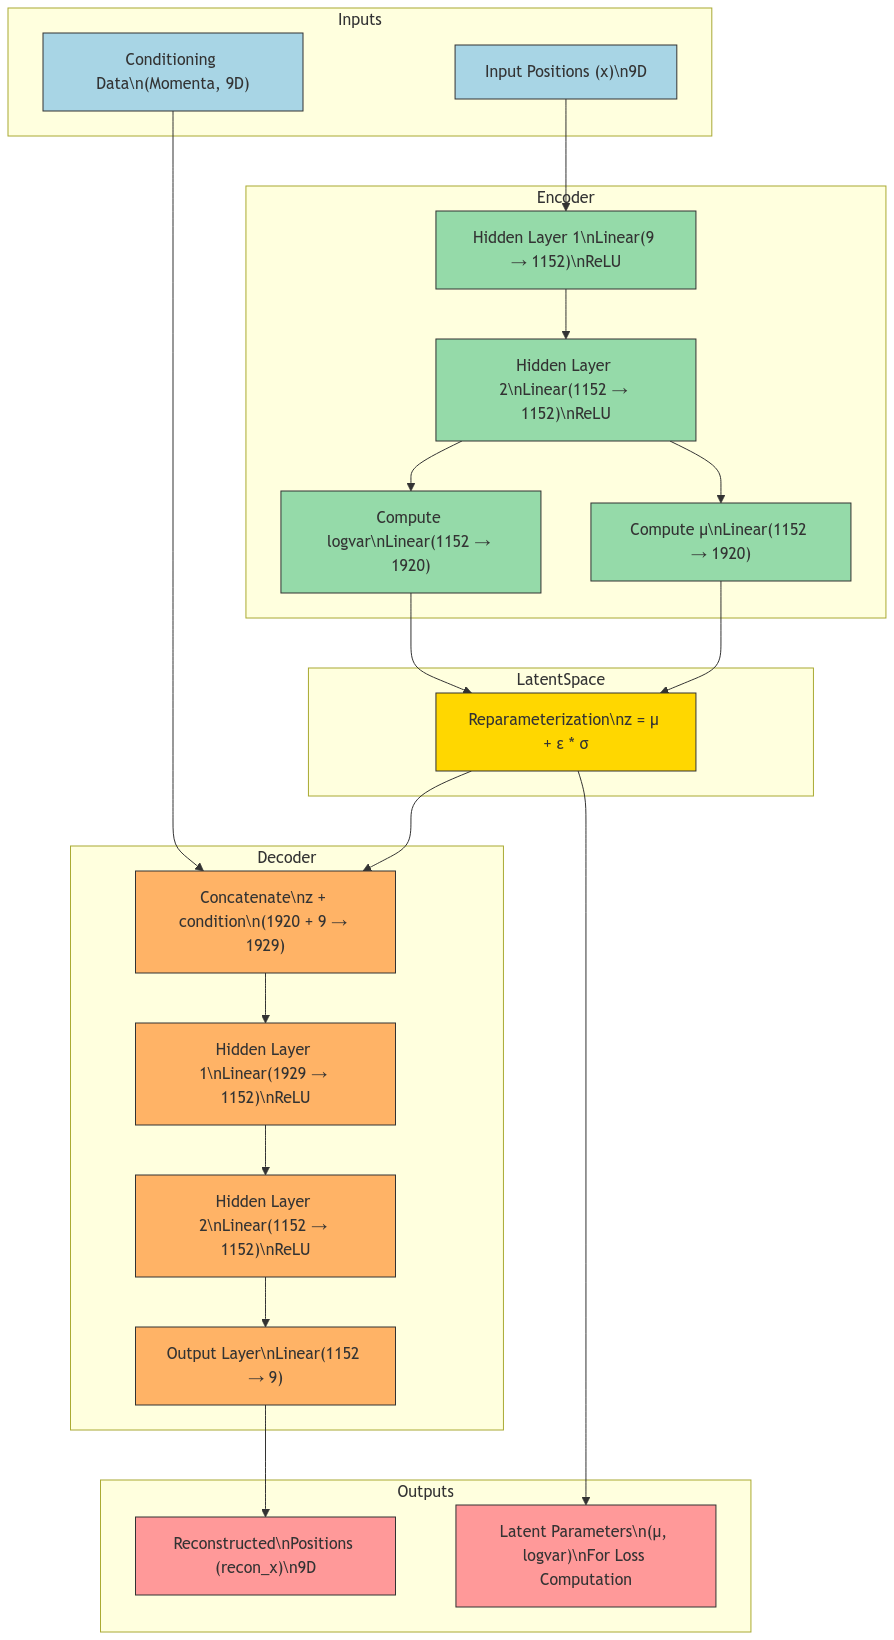
\includegraphics[width=0.8\textwidth]{4.png}
    \caption{Complete System Architecture: Detailed block diagram showing the entire system organization, including input processing, encoder-decoder structure, latent space operations, and output generation with explicit dimensionality annotations for each transformation.}
    \label{fig:system}
\end{figure}

\section{Implementation Features}

\subsection{Activation Functions}
\begin{itemize}
    \item \textbf{ReLU in Hidden Layers:}
    \begin{itemize}
        \item Function: $f(x) = \max(0, x)$
        \item Prevents vanishing gradients
        \item Promotes sparse activation
    \end{itemize}
    \item \textbf{Linear Output Layer:}
    \begin{itemize}
        \item Enables unbounded reconstruction
        \item Preserves continuous value ranges
        \item Suitable for regression tasks
    \end{itemize}
\end{itemize}

\subsection{Layer Configuration}
\begin{itemize}
    \item \textbf{Dimensionality:}
    \begin{itemize}
        \item Input dimension: 9 (position vectors)
        \item Hidden layers: 1152 neurons
        \item Latent dimension: 1920
    \end{itemize}
    \item \textbf{Architecture:}
    \begin{itemize}
        \item Symmetric design between encoder and decoder
        \item Progressive dimension transformation
        \item Careful capacity allocation
    \end{itemize}
\end{itemize}

\section{Training Results}

\subsection{Training Progress}
\begin{table}[H]
\centering
\begin{tabular}{ll}
\toprule
\textbf{Metric} & \textbf{Value} \\
\midrule
Epoch & 45 \\
CVAE loss & $1.0619$ \\
Validation loss & $0.9250$ \\
\bottomrule
\end{tabular}
\caption{Training progress metrics}
\label{tab:training_progress}
\end{table}

\medskip

Early stopping CVAE training after 45 epochs.

\subsection{Test Set Evaluation}
\begin{table}[H]
\centering
\begin{tabular}{ll}
\toprule
\textbf{Metric} & \textbf{Value} \\
\midrule
Test MSE & $0.7208$ \\
Mean Relative Error & $0.6860$ \\
\bottomrule
\end{tabular}
\caption{Test set evaluation metrics}
\label{tab:test_evaluation}
\end{table}

\medskip

\subsection{Cross-Validation Results}
\begin{table}[H]
\centering
\begin{tabular}{lcr}
\toprule
\textbf{Fold} & \textbf{Test MSE} & \textbf{Mean Relative Error} \\
\midrule
1 & $0.7939$ & $1.6674$ \\
2 & $0.7829$ & $1.0861$ \\
3 & $0.7676$ & $1.1567$ \\
4 & $0.7695$ & $0.9325$ \\
5 & $3.6450$ & $5.5142$ \\
\midrule
\textbf{Average} & $1.3518 \pm 1.1467$ & $2.0714 \pm 1.7390$ \\
\bottomrule
\end{tabular}
\caption{Cross-validation results across 5 folds}
\label{tab:cross_validation}
\end{table}

\subsection{Training Loss Evolution}
\begin{figure}[H]
    \centering
    \subfigure[First 10 Epochs]{
        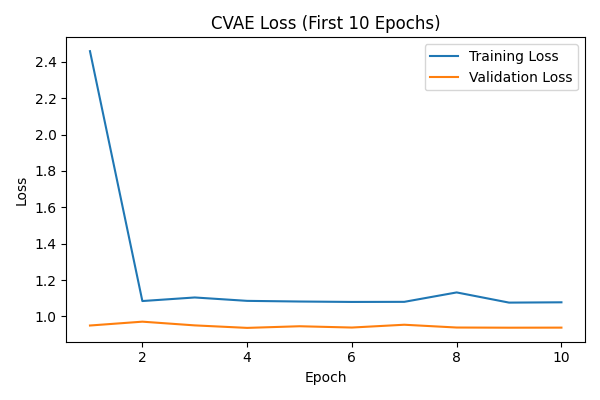
\includegraphics[width=0.48\textwidth]{cvae_loss_plot_first10_CINNV4.png}
        \label{fig:first10}
    }
    \subfigure[Remaining Epochs]{
        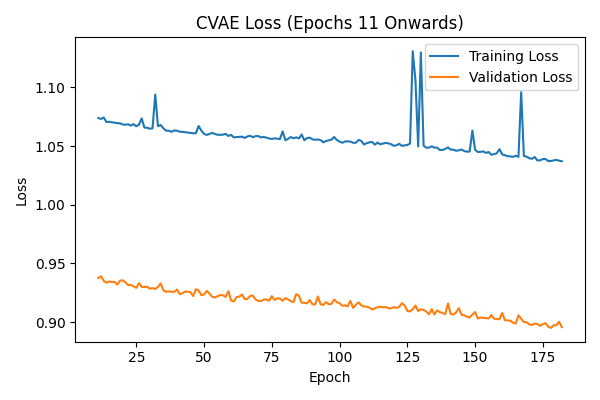
\includegraphics[width=0.48\textwidth]{cvae_loss_plot_rest_CINNV4.png}
        \label{fig:remaining}
    }
    \caption{CVAE Training Loss Evolution: (a) Initial rapid convergence in the first 10 epochs, showing dramatic loss reduction from 2.4 to 1.1; (b) Long-term training behavior from epoch 11 onwards, demonstrating stable training loss around $1.05$ and gradually improving validation loss.}
    \label{fig:learning_curves}
\end{figure}

\subsection{Analysis of Training Performance}
The training process exhibits several notable characteristics:

\begin{itemize}
    \item \textbf{Initial Convergence:}
    \begin{itemize}
        \item Rapid loss reduction in the first two epochs ($2.4 \rightarrow 1.1$)
        \item Quick stabilization of both training and validation losses
    \end{itemize}
    
    \item \textbf{Long-term Behavior:}
    \begin{itemize}
        \item Training loss maintains steady state around $1.05$
        \item Validation loss shows consistent improvement ($0.94 \rightarrow 0.90$)
        \item Occasional training loss spikes indicating potential optimization challenges
    \end{itemize}
    
    \item \textbf{Cross-validation Performance:}
    \begin{itemize}
        \item Consistent performance across folds 1-4 (MSE $\approx$ $0.77$-$0.79$)
        \item Significant deviation in fold 5 (MSE = $3.6450$)
        \item Higher variability in mean relative error compared to MSE
    \end{itemize}
    
    \item \textbf{Early Stopping:}
    \begin{itemize}
        \item Training terminated at epoch 45
        \item Final CVAE loss: $1.0619$
        \item Final validation loss: $0.9250$
    \end{itemize}
\end{itemize}

The cross-validation results (Table~\ref{tab:cross_validation}) reveal generally consistent performance across most folds, with an anomalous performance in fold 5. This suggests potential sensitivity to data partitioning that may require further investigation.

\section{Conclusion}
The implemented CVAE architecture demonstrates a sophisticated approach to conditional generative modeling, particularly suited for position-momentum relationships. The training results show effective convergence and generally stable performance, with the following key characteristics:

\begin{itemize}
    \item High-dimensional latent space for complex pattern capture
    \item Effective conditioning mechanism
    \item Deep network structure for sophisticated transformations
    \item Robust sampling through reparameterization
    \item Consistent performance across most cross-validation folds
\end{itemize}

Future work could explore:
\begin{itemize}
    \item Investigation of fold 5 anomalies
    \item Alternative conditioning mechanisms
    \item Dynamic latent space dimensionality
    \item Advanced regularization techniques
    \item Hybrid architecture variations
\end{itemize}

\section{Regularization}

Evaluating on test set...\\
Test MSE: 0.7302\\
Mean Relative Error: 0.6690

\begin{itemize}[leftmargin=*]
\item \textbf{Dropout Regularization:}
  \begin{itemize}
    \item Introduce \texttt{nn.Dropout} layers in both the encoder and decoder networks. Dropout randomly deactivates a subset of neurons during training, which helps in preventing overfitting by ensuring that the network doesn't become overly reliant on any particular neuron.
  \end{itemize}

\item \textbf{Early Stopping Refinement:}
  \begin{itemize}
    \item Implement a more robust early stopping mechanism that not only considers the validation loss but also tracks improvements over a specified patience period.
  \end{itemize}

\item \textbf{Additional Improvements:}
  \begin{itemize}
    \item \textbf{Batch Normalization (Optional):} While not explicitly requested, batch normalization can further stabilize and accelerate training. You can uncomment the related sections if you wish to include it.
    \item \textbf{Logging Enhancements:} Improved logging for better monitoring of training progress.
  \end{itemize}
\end{itemize}
\end{document}
